\newpage
\section{Progettazione}
\subsection{Studio dell'utenza finale}
\subsubsection{Utente generico}
L'utente generico che in generale visiterà il sito è di profilo informatico medio alto ed è alla ricerca di informazioni riguardanti serie TV.
L'utente generico non registrato ha a disposizione le seguenti azioni:
\begin{itemize}
	\item eseguire il \textit{login} oppure effettuare l'\textit{iscrizione} al sito;
	\item navigare nelle pagine \textit{homepage, esplora, serie TV, FAQ, supporto, privacy} e \textit{about};
	\item effettuare la ricerca di serie TV grazie alla casella di ricerca presente nella barra di navigazione.
\end{itemize}
Qualora l'utente non registrato tentasse di utilizzare le funzionalità riservate agli utenti registrati, verrà reindirizzato alla pagina di accesso o registrazione.

L'utente generico registrato ha a disposizione le seguenti azioni:
\begin{itemize}
	\item eseguire il \textit{logout};
	\item navigare nelle pagine \textit{homepage, esplora, serie TV, preferiti, FAQ, supporto, privacy} e \textit{about};
	\item all'interno della pagina dedicata alle singole serie TV, l'utente potrà:
	\begin{itemize}
		\item consigliare o meno la serie;
		\item votare la serie con una valutazione da 1 a 5;
		\item aggiungere la serie ai preferiti; 
		\item creare post e partecipare a discussioni;
		\item segnalare i commenti inappropriati degli altri utenti;
		\item segnare una serie TV come visualizzato o non visualizzata.
	\end{itemize}
\end{itemize}


\subsubsection{Amministratore}
I permessi aggiunti agli utenti amministratori permettono di accedere alla pagina di amministrazione.\\
All'interno dell'area dedicata all'amministrazione è possibile svolgere le seguenti attività:
\begin{itemize}
	\item visualizzare in forma tabellare i commenti segnalati dagli utenti. Sarà possibile decidere di ignorare la segnalazione oppure di eliminare il commento segnalato, inoltre ha la possibilità di non far vedere un commento esclusivamente all'utente che l'ha segnalato;
	\item visualizzare in forma tabellare i messaggi ricevuti dagli utenti, inviati dall'apposita sezione "Supporto", e decidere di dare una risposta oppure di eliminare i messaggi.
\end{itemize}
Qui di seguito è riportata la schermata che si presenta all'utente amministratore:
\begin{figure}[h!]
	\centerline{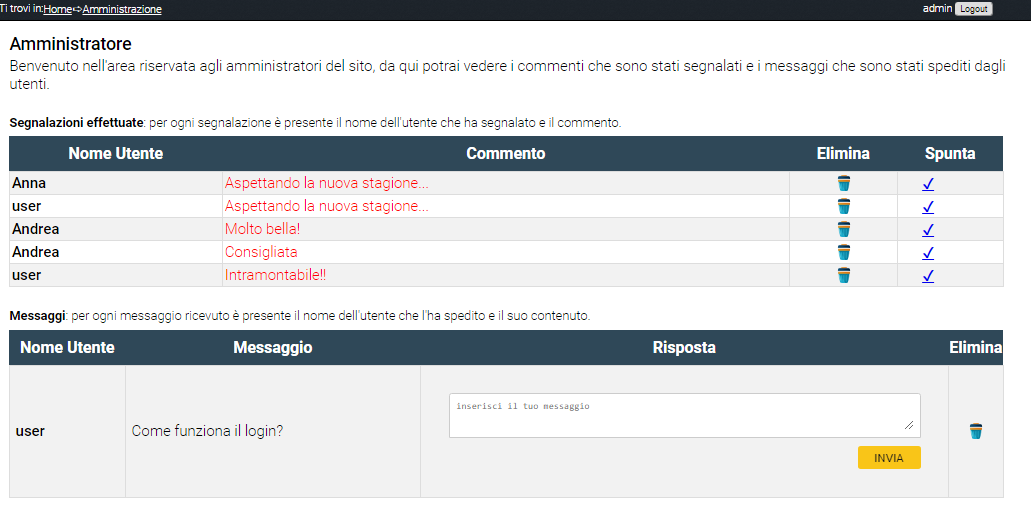
\includegraphics[scale=0.45]{img/amministratore.png}}
	\caption{Pagina amministratore in modalità desktop}
	\label{fig:navbarGU}
\end{figure}


\subsection{Layout del sito}
Il sito TV Hunter è stato sviluppato con l'approccio \textit{mobile first}. Lo stile definito nei file .css è quindi strutturato nel seguente modo:
\begin{itemize}
	\item regole di stile per la versione mobile del sito;
	\item regole di stile in una \textit{media query} per i dispositivi tablet (min-width 751px max-width 1024px);
	\item regole di stile in una \textit{media query} per schermi desktop (min-width 1025px).
\end{itemize}
Vengono di seguito presentate prima le componenti principali del layout e successivamente le pagine principali del sito TV Hunter. \\
Per ogni pagina o componente sono evidenziate le scelte più interessanti relative allo stile, alla struttura delle pagine, nonchè al comportamento.

\subsubsection{Barra di navigazione}
Che ci si trovi in modalità mobile, tablet o desktop, si potrà navigare all'interno del sito tramite il menù o la barra di navigazione che è sempre resa disponibile nella forma migliore in base alla situazione.\\
\begin{itemize}
	\item In \textbf{modalità mobile} La barra di navigazione ed il menù sono divisi. La barra di navigazione si trova sulla parte superiore della pagina. Da qui sarà possibile usare la casella di ricerca oppure, tramite il link \textit{Menu} sarà possibile visualizzare le voci del menù presenti sul fondo della pagina.\\
	Questa scelta permette di evitare l'uso di JavaScript per la visualizzazione del menu. Il tasto \textit{Menu} risulta inoltre più intuitivo dell'immagine "ad hamburger" spesso utilizzata per la visualizzazione dei menù mobile che potrebbe rivelarsi disorientante per l'utenza con meno esperienza.\\
	Sul fondo della pagina è presente il link \textit{Torna su} che permette di tornare facilmente a visualizzare le informazioni contenute nella pagina;
	
	\item In \textbf{modalità tablet} la barra di navigazione è divisa in maniera simile alla modalità mobile: sulla parte superiore della pagina è presente la barra con logo, casella di ricerca e tre voci del menù. Nella barra posta sul fondo a piè di pagina sono presenti le voci rimanenti (quelle secondarie) del menù. \\
	Entrambe le barre sono posizionate in maniera \textit{fissa}. La barra superiore ha una altezza fissata in \textit{em}.\\
	
	\item In \textbf{modalità desktop} la barra di navigazione è posta in verticale sul lato sinistro. Questa ha una \textit{larghezza} del 20\% ed è posta in \textit{posizione} fissa.\\
	Nel menù sono elencate le voci principali (\textit{esplora, profilo, preferiti}) nel primo blocco e le voci secondarie (\textit{FAQ, supporto, privacy, about}) in un secondo blocco.\\
	Alla sinistra delle voci, grazie al selettore \textit{:before}, sono state inserite delle icone che aiutano ad individuare più rapidamente la voce che si sta cercando.\\
	Nel menù laterale sulla parte superiore è presente lo spazio per la ricerca delle serie tv.
\end{itemize}
	La voce del menù relativa alla pagina in cui ci si trova è evidenziata di colore bianco e non sarà cliccabile per evitare link che puntano alla pagina in cui ci si trova.
	Sarà poi possibile capire dove ci si trovi all'interno del sito grazie al percorso indicato sulla barra sempre presente nella parte superiore della pagina.

\begin{figure}[H]
	\centerline{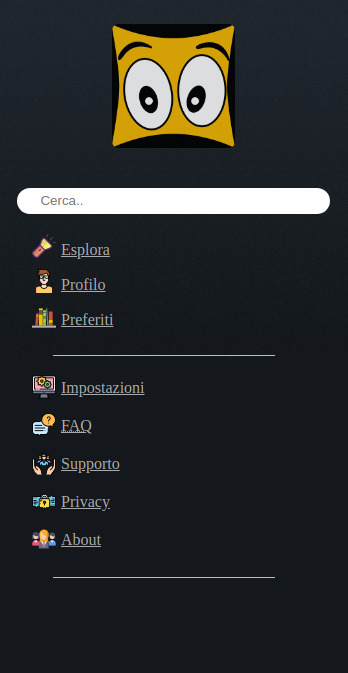
\includegraphics[scale=0.45]{img/nav_bar.png}}
	\caption{Barra di navigazione per utente generico in modalità desktop}
	\label{fig:navbarGU}
\end{figure}

\subsubsection{Barra informativa}
Posizionata sotto l'header si trova la barra informativa.\\
In caso di accesso effettuato viene indicato sul lato destro l'username dell'utente ed è presente il pulsante per effettuare la disconnessione.\\
In caso di utente non autenticato è disponibile il pulsante per effettuare il login, che rimanderà alla pagina di autenticazione.\\
Sulla parte sinistra, nelle versioni mobile e tablet viene indicato il percorso effettuato per arrivare alla pagina corrente, con la possibilità di muoversi all'indietro. 


\paragraph{Contenuti statici}

\paragraph{About} 
~\\	
La pagina di \textit{about} contiene informazioni riguardanti la piattaforma e i membri del gruppo con le relative foto. 
\begin{figure}[H]
	\centerline{
\includegraphics[scale=0.33]{img/about.png}}
	\caption{Pagina di About in modalità desktop}
	\label{fig:addForm} 
\end{figure}	

\paragraph{Privacy} 
~\\	
La pagina di \textit{privacy} contiene le linee guida adottate dalla piattaforma per il trattamento dei dati personali degli utenti registrati.
\begin{figure}[h!]
	\centerline{
\includegraphics[scale=0.23]{img/privacy.png}}
	\caption{Pagina di Privacy in modalità desktop}
	\label{fig:addForm} 
\end{figure}	

\paragraph{Contenuti dinamici}   

\subparagraph{Preferiti}
~\\	
La pagina di \textit{preferiti} raccoglie le serie TV che sono state selezionate come preferite dall'utente in modo che in futuro non debba ricercarle nuovamente. Le serie salvate vengono mostrate in modo ordinato e se non sono presenti serie TV preferite viene visualizzata una pagina vuota. 
\begin{figure}[H]
	\centerline{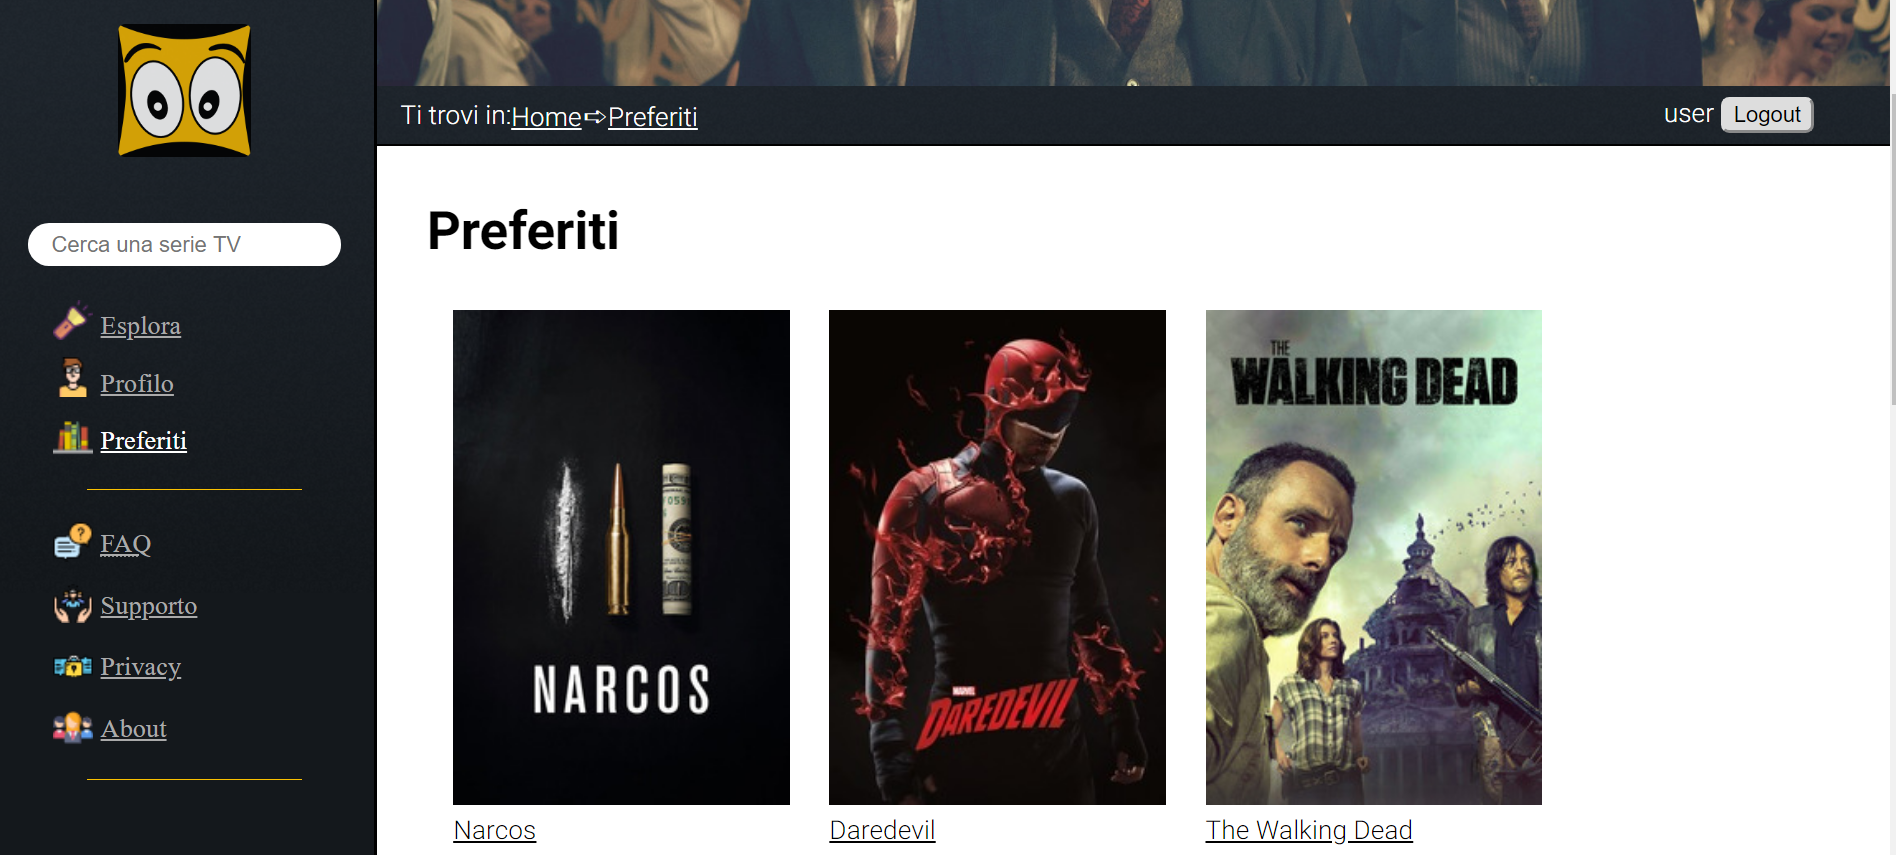
\includegraphics[scale=0.33]{img/preferiti.png}}
	\caption{Pagina di Preferiti in modalità desktop}
	\label{fig:addForm}
\end{figure}	


\subparagraph{Esplora}
~\\	
La pagina di \textit{esplora} elenca per genere le serie TV che il sito ha nel database. Ogni genere ha il 100\% di spazio in larghezza a disposizione ma qualora questo spazio non dovesse bastare a mostrare tutte le serie appartenenti al genere, l'utente potrà comunque visualizzarle tutte in una pagina dedicata, raggiungibile tramite il link \textit{mostra tutto} presente sul lato destro dell'elenco delle serie.
\begin{figure}[H]
	\centerline{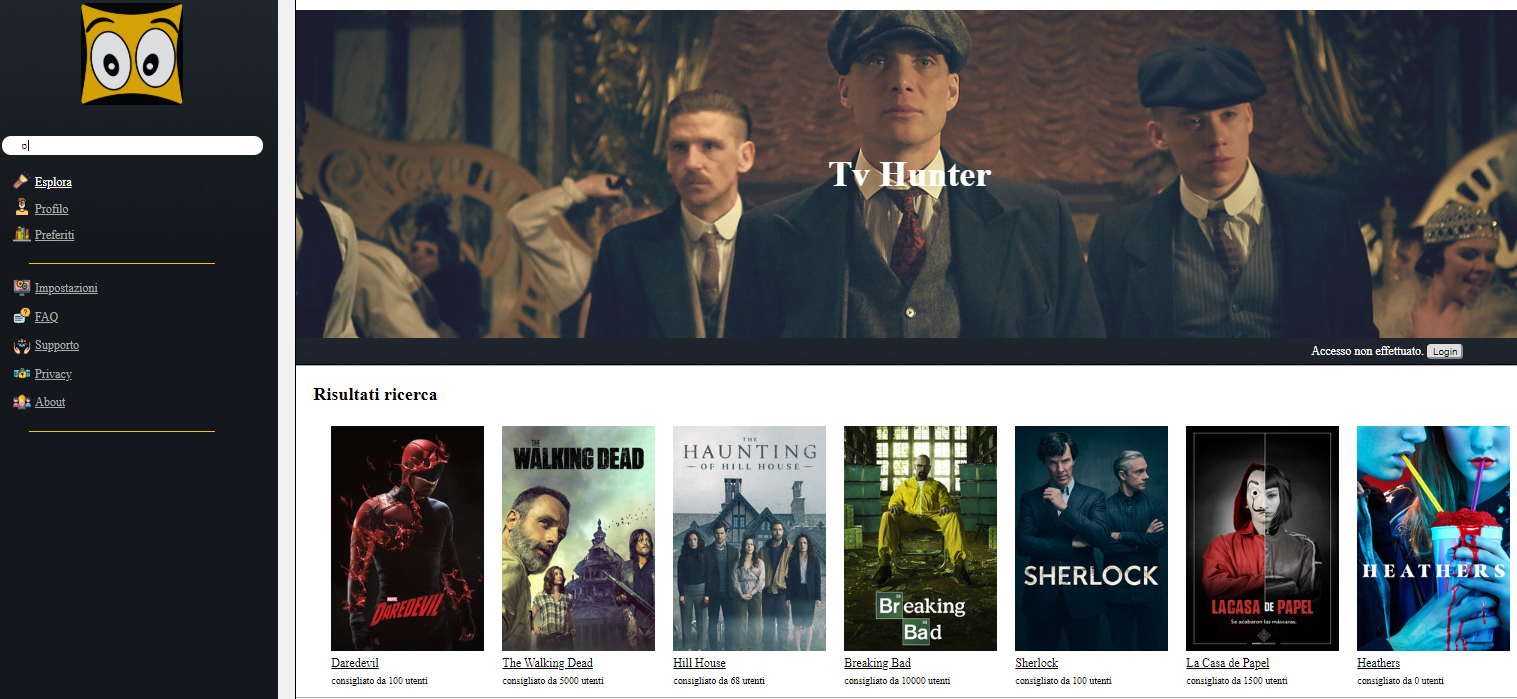
\includegraphics[scale=0.33]{img/esplora.png}}
	\caption{Pagina esplora in modalità desktop}
	\label{fig:addForm}
\end{figure}	

\subparagraph{Profilo}
~\\
La pagina di \textit{profilo} presenta: nome, cognome, data di nascita, username e la Email dell'utente registrato. In caso di mancata registrazione il sistema mostrerà una schermata dove darà, tramite un link, la possibilità di registrarsi o di autenticarsi come utente registrato nell'apposita pagina di registrazione. 
\begin{figure}[H]
	\centerline{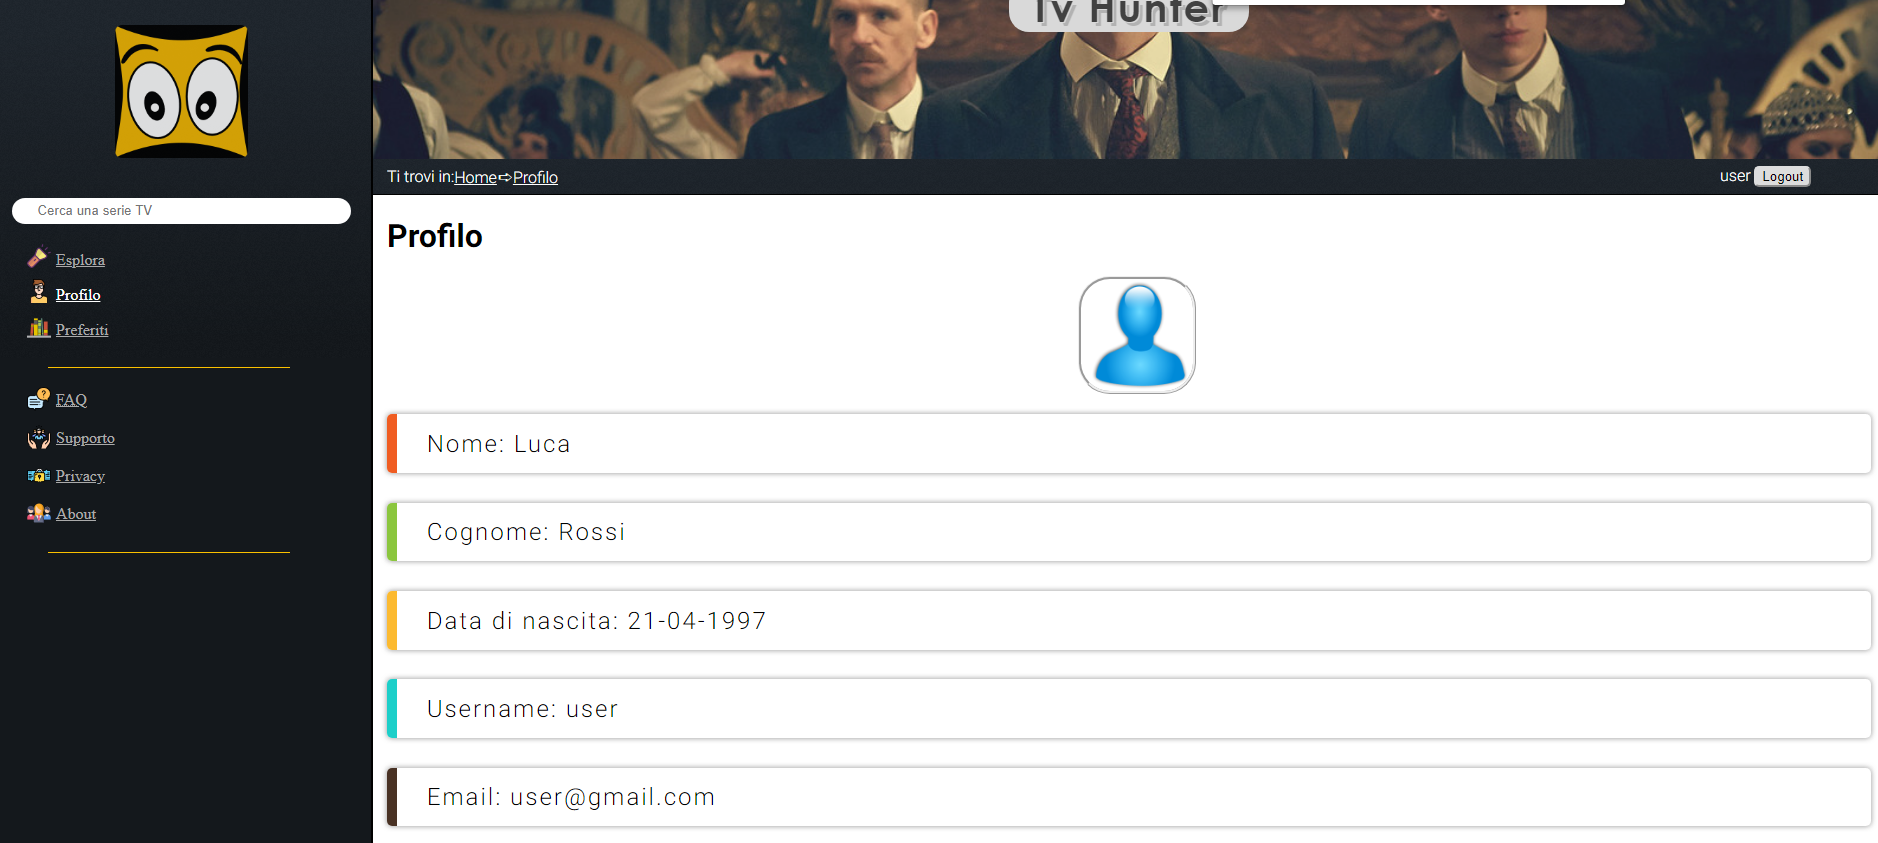
\includegraphics[scale= 0.33]{img/profilo.png}}
	\caption{Pagina Profilo in modalità desktop}
\end{figure}


\subparagraph{FAQ} 
~\\
La pagina di \textit{faq} presenta le domande che più sono state richieste dagli utenti registrati agli amministratori con le relative risposte. Inoltre per ogni domanda è presente, se necessaria, un'immagine che indica il posizionamento delle \textit{"aree"} del sito che possono non essere state trovate.
\begin{figure}[H]
	\centerline{
\includegraphics[scale= 0.33]{img/faq.png}}
	\caption{Pagina Faq in modalità desktop}
	
\end{figure}


\subparagraph{Serie}
~\\
La pagina di \textit{serie} contiene le informazioni riguardanti una serie TV specifica, il titolo delle serie TV è posto in cima alla pagina e viene caricata l'immagine della serie nell'\textit{head}. È poi presente una sezione \textit{Post} che permette di lasciare un commento che, se inviato, sarà reso visibile agli utenti o visitatori del sito. A lato della pagina è possibile aggiungere la serie ai \textit{preferiti} e viene data la possibilità di selezionare un voto da uno a cinque e di lasciare un \textit{feedback} positivo o negativo tramite la selezione del pollice rivolto in su o in giù. 

\begin{figure}[H]
	\centerline{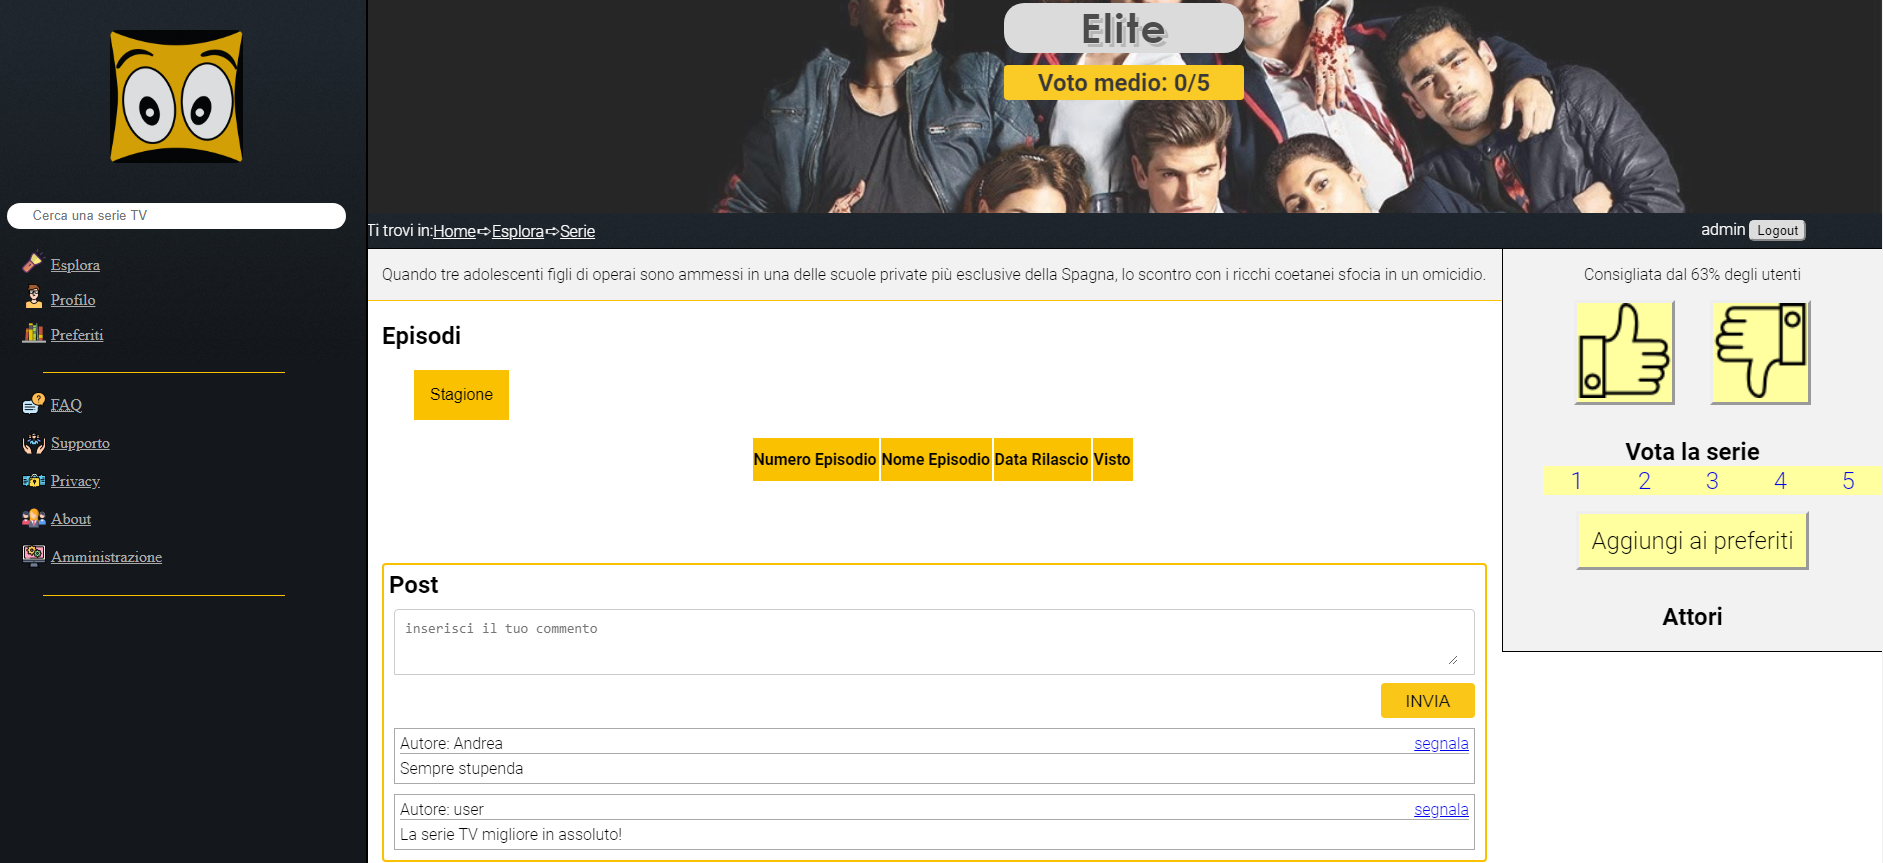
\includegraphics[scale= 0.33]{img/serie.png}}
	\caption{Pagina serie in modalità desktop}
	
\end{figure}

